% Boilerplate from: https://github.com/jdavis/latex-homework-template/blob/master/homework.tex
\documentclass[table]{article}
\usepackage[table]{xcolor}
\usepackage{amssymb}
\usepackage{fancyhdr}
\usepackage{extramarks}
\usepackage{amsmath}
\usepackage{amsthm}
\usepackage{amsfonts}
\usepackage{tikz}
\usepackage{graphicx}
\usepackage{enumitem}


\topmargin=-0.45in
\evensidemargin=0in
\oddsidemargin=0in
\textwidth=6.5in
\textheight=9.0in
\headsep=0.25in

\linespread{1.1}
\pagestyle{fancy}
\lhead{\hmwkAuthorName}
\chead{\hmwkTitle}
\rhead{\firstxmark}
\lfoot{\lastxmark}
\cfoot{\thepage}

\renewcommand\headrulewidth{0.4pt}
\renewcommand\footrulewidth{0.4pt}

%\setlength\parindent{15pt}%

\newcommand{\enterProblemHeader}[1]{
    \nobreak\extramarks{}{Problem \arabic{#1} continued on next page\ldots}\nobreak{}
    \nobreak\extramarks{Problem \arabic{#1} (continued)}{Problem \arabic{#1} continued on next page\ldots}\nobreak{}
}

\newcommand{\exitProblemHeader}[1]{
    \nobreak\extramarks{Problem \arabic{#1} (continued)}{Problem \arabic{#1} continued on next page\ldots}\nobreak{}
    \stepcounter{#1}
    \nobreak\extramarks{Problem \arabic{#1}}{}\nobreak{}
}

\setcounter{secnumdepth}{0}
\newcounter{partCounter}
\newcounter{homeworkProblemCounter}
\setcounter{homeworkProblemCounter}{1}
\nobreak\extramarks{Problem \arabic{homeworkProblemCounter}}{}\nobreak{}

\newenvironment{homeworkProblem}[1][-1]{
    \ifnum#1>0
        \setcounter{homeworkProblemCounter}{#1}
    \fi
    \section{Problem \arabic{homeworkProblemCounter}}
    \setcounter{partCounter}{1}
    \enterProblemHeader{homeworkProblemCounter}
}{
    \exitProblemHeader{homeworkProblemCounter}
}

\newcommand{\hmwkTitle}{Homework\ \#1}
\newcommand{\hmwkDueDate}{22 June 2020}
\newcommand{\hmwkClass}{Discrete Structures}
\newcommand{\hmwkClassTime}{Section 201}
\newcommand{\hmwkClassInstructor}{Professor Jensen}
\newcommand{\hmwkAuthorName}{\textbf{Brian Ton}}

\title{
    \vspace{2in}
    \textmd{\textbf{\hmwkClass:\ \hmwkTitle}}\\
    \normalsize\vspace{0.1in}\small{Due\ on\ \hmwkDueDate}\\
    \vspace{0.1in}\large{\textit{\hmwkClassInstructor\ \hmwkClassTime}}
    \vspace{3in}
}

\author{\hmwkAuthorName}
\date{}

\newcommand{\solution}{\textbf{\large Solution}}

\newcolumntype{g}{>{\columncolor{yellow!20}}c}

\begin{document}
\maketitle

\pagebreak

\begin{homeworkProblem}
	True or False: The statements \emph{``If Earl studied, then Earl received an A.''} and \emph{``If Earl received an A, then Earl studied.''} are logically equivalent.
	
	\subsection{\textbf{Solution}}
	\textbf{False}\\
	Here, the two statements are converses of each other, which are not logically equivalent.\\~\\
	For instance, consider the situation where Earl got an A but did not study. In this instance, the original statement is true because Earl did not satisfy the hypothesis. However, the second statement would be false because Earl got an A without studying. Thus, the two statements are not logically equivalent.
\end{homeworkProblem}
\begin{homeworkProblem}
	True or False: The statements \emph{``If Earl studied, then Earl received an A.''} and \emph{``If Earl did not
receive an A, the Earl did not study.''} are logically equivalent.
	\subsection{\textbf{Solution}}
	\textbf{True}\\%
	Here, the two statements are contrapositives of each other, which are logically equivalent.\\~\\
	Let \(p\) be the proposition \emph{``Earl studied''} and \(q\) be the proposition \emph{``Earl recieved an A.''}. Note that the first statement given in the problem can be rewritten using the above statements as \(p{\rightarrow}q\), and the second statement given in the problem as \({\neg}q{\rightarrow}{\neg}p\). The truth table for each statement given in the problem is the following:
\begin{displaymath}
\begin{array}{|c c|c|c|}
% |c c|c| means that there are three columns in the table and
% a vertical bar ’|’ will be printed on the left and right borders,
% and between the second and the third columns.
% The letter ’c’ means the value will be centered within the column,
% letter ’l’, left-aligned, and ’r’, right-aligned.
p & q & p \rightarrow q & {\neg}q {\rightarrow} {\neg} p\\ % Use & to separate the columns
\hline % Put a horizontal line between the table header and the rest.
T & T & T & T\\
T & F & F & F\\
F & T & T & T\\
F & F & T & T\\
\end{array}
\end{displaymath}
Since \({\neg}q{\rightarrow}{\neg}p{\:}{\equiv}{\:}p{\rightarrow}q\), the statements \emph{``If Earl studied, then Earl received an A.''} and \emph{``If Earl did not
receive an A, the Earl did not study.''} are logically equivalent.
\end{homeworkProblem}
\begin{homeworkProblem}
Write the negation of the statement \emph{``If Earl studied, then Earl received an A.''}
\subsection{\textbf{Solution}}
	\textbf{\emph{Earl studied and did not receive an A}}\\~\\
Let \(p\) be the proposition \emph{``Earl studied''} and \(q\) be the proposition \emph{``Earl recieved an A.''} Note that \({\neg}(p{\rightarrow}q){\:}{\equiv}{\:}p{\land}{\neg}q\). Thus we can write the negation of \emph{``If Earl studied, then Earl received an A.''} as \emph{``Earl studied and did not receive an A''}.
\end{homeworkProblem}
\begin{homeworkProblem}
Write the converse, inverse, and contrapositive of the statement \emph{``If Popeye is a Dachshund, then Popeye has short legs.''}
\subsection{\textbf{Solution}}
\textbf{Converse: \emph{``If Popeye has short legs, then Popeye is a Dachshund''}}\\
\textbf{Inverse: \emph{``If Popeye is not a Dachshund, then Popeye does not have short legs''}}\\
\textbf{Contrapositive: \emph{``If Popeye does not have short legs, then Popeye is not a Dachshund''}}\\~\\
Let \(p\) be the proposition \emph{``Popeye is a Dachshund''} and \(q\) be the proposition \emph{``Popeye has short legs''}. Note that the converse of \(p{\rightarrow}q\) is defined as \(q{\rightarrow}p\), the inverse of \(p{\rightarrow}q\) is defined as \({\neg}p{\rightarrow}{\neg}q\), and the contrapositive of \(p{\rightarrow}q\) is defined as \({\neg}q{\rightarrow}{\neg}p\). Thus, the converse of the original statement is \emph{``If Popeye has short legs, then Popeye is a Dachshund,''} the inverse of the original statement is \emph{``If Popeye is not a Dachshund, then Popeye does not have short legs,''} and the contrapositive of the original statement is \emph{``If Popeye does not have short legs, then Popeye is not a Dachshund.''}
\end{homeworkProblem}
\begin{homeworkProblem}
Use a truth table to determine whether \((p{\land}{\neg}q){\rightarrow}r{\:}{\equiv}{\:}p{\rightarrow}(q{\lor}r)\).
\subsection{\textbf{Solution}}
\textbf{True}\\~\\
\begin{displaymath}
\begin{array}{|c c c|c|g|c|g|}
% |c c|c| means that there are three columns in the table and
% a vertical bar ’|’ will be printed on the left and right borders,
% and between the second and the third columns.
% The letter ’c’ means the value will be centered within the column,
% letter ’l’, left-aligned, and ’r’, right-aligned.
p & q & r & p{\land}{\neg}q & (p{\land}{\neg}q){\rightarrow}r & q{\lor}r &  p{\rightarrow}(q{\lor}r)\\
\hline
T & T & T & F & T & T & T\\
T & T & F & F & T & T & T\\
T & F & T & T & T & T & T\\
T & F & F & T & F & F & F\\
F & T & T & F & T & T & T\\
F & T & F & F & T & T & T\\
F & F & T & F & T & T & T\\
F & F & F & F & T & F & T\\
\end{array}
\end{displaymath}
In the above, since column \((p{\land}{\neg}q){\rightarrow}r\) and \(p{\rightarrow}(q{\lor}r)\) (both highlighted) have matching corresponding elements, \((p{\land}{\neg}q){\rightarrow}r{\:}{\equiv}{\:}p{\rightarrow}(q{\lor}r)\). Without building the truth table, this can still be justified.\\
Note that \(p{\land}{\neg}q\) can only be true when \(p\) is true and \(q\) is false, which means that the statement \((p{\land}{\neg}q){\rightarrow}r\) can only be false when \(p\) is true, \(q\) is false, and \(r\) is false (which gives the implication \(T{\rightarrow}F\) which is logically equivalent to \(F\)). Using similar reasoning, since \(a{\rightarrow}b\) is only false when \(a\) is true and \(b\) is false, \(p{\rightarrow}(q{\land}r)\) is false when p is true and \(q{\land}r)\) is false, which is only true where \(q\) and \(r\) are both false. Thus, since they are both only false where \(p\) is true and both \(q\) and \(r\) are false and true otherwise, the two statements must be logically equivalent.
\end{homeworkProblem}
\pagebreak
\begin{homeworkProblem}
Let \(p\), \(q\), and \(r\) be the propositions\\
\indent{\(p\):\emph{``You get an A on the final exam''}}\\%
\indent{\(q\):\emph{``You do every exercise in this book''}}\\
\indent{\(r\):\emph{``You get an A in this class''}}\\
Write these statements using \(p\), \(q\), \(r\) and logical connectives (including negations).
\begin{enumerate}[nosep, label=\textbf{\alph*})]
\item You get an A in this class, but you do not do every exercise in this book.
\item You get an A on the final, you do every exercise in this book, and you get an A in this class.
\item To get an A in this class, it is necessary for you to get an A on the final.
\item You get an A on the final, but you don't do every exercise in this book; nevertheless, you get an A in this class.
\item Getting an A on the final and doing every exercise in this book is sufficient for getting an A in this class.
\item You will get an A in this class if and only if you either do every exercise in this book or you get an A on the final.
\end{enumerate}
\subsection{\textbf{Solution}}
\begin{enumerate}[nosep, label=\textbf{\alph*})]
\item \(p{\land}{\neg}q\)
\item \(p{\land}q{\land}r\)
\item \(r{\rightarrow}p\)
\item \(p{\land}{\neg}q{\land}r\) (Note that the statement can be rewritten as ``You get an A on the final, do not do every exercise \textit{and} you get an A in this class'', as in this case, the word \textit{and} can replace \textit{nevertheless} without changing the meaning)
\item \((p{\land}q){\rightarrow}r\)
\item \(r{\iff}(q{\lor}p)\)
\end{enumerate}
\end{homeworkProblem}
\pagebreak
\begin{homeworkProblem}
Find the output of each of these combinatorial circuits
\begin{figure}[h!]
	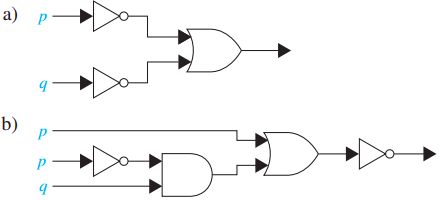
\includegraphics[scale=.75]{images/Prob7FigureUnannotated.png}
\end{figure}
\subsection{\textbf{Solution}}
\begin{enumerate}[nosep, label=\textbf{\alph*})]
\item \({\neg}p{\lor}{\neg}q\)
\item \({\neg}(p{\lor}({\neg}p{\land}q))\)\\
\end{enumerate}
(Annotated Figures)
\begin{figure}[h!]
	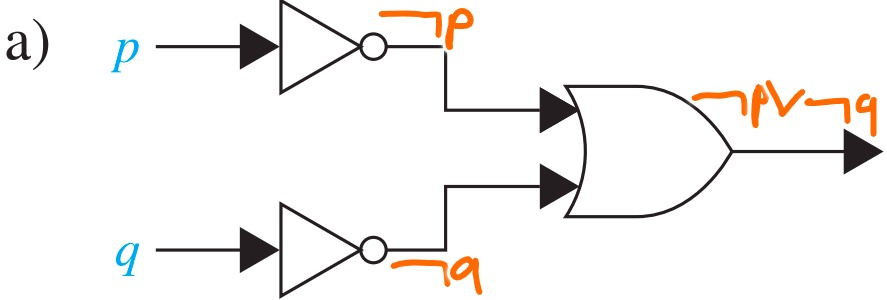
\includegraphics[scale=.25]{images/Prob7FigureAAnnotated.jpeg}
\end{figure}
\begin{figure}[h!]
	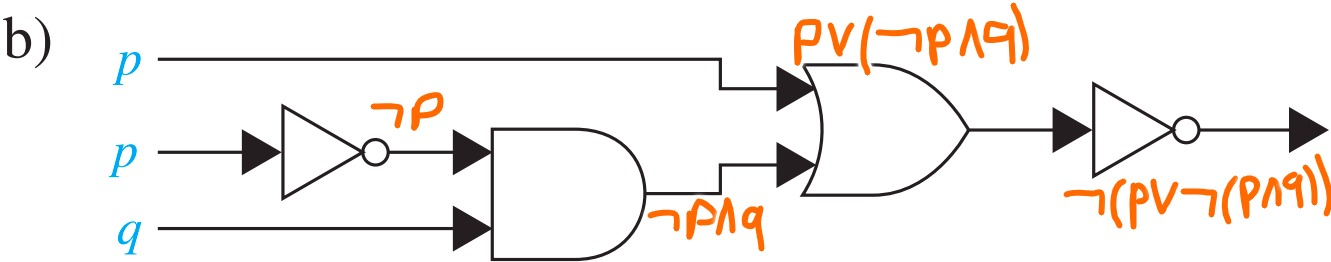
\includegraphics[scale=.25]{images/Prob7FigureBAnnotated.jpeg}
\end{figure}
\end{homeworkProblem}
\pagebreak
\begin{homeworkProblem}
Construct a combinatorial circuit using inverters, OR gates, and AND gates that produces the output \((p{\land}{\neg}r){\lor}({\neg}q{\land}r)\) from the input bits \(p\), \(q\), and \(r\).
\subsection{\textbf{Solution}}
\begin{figure}[h!]
	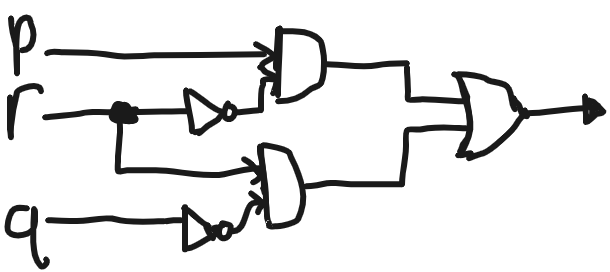
\includegraphics[scale=.35]{images/Prob8Solution.jpeg}
\end{figure}
\end{homeworkProblem}
\begin{homeworkProblem}
A says “The two of us are both knights” and B says “A is
a knave.”
\subsection{\textbf{Solution}}
\emph{\textbf{A is a Knave\\ B is a Knight}}\\~\\
Assume A is a knight. As a result, B must also be a knight. However, if B is a knight as well, A cannot be a knight, as then B would be lying.\\
A must then be a knave. As a result, B must be a knight, as he is telling the truth in this instance. Note that when A is a knave and B is a knight, both satisfy the requirements of the problem, as A is not telling the truth (as both of them are not knights) and B is telling the truth (as A is a knave).
\end{homeworkProblem}
\begin{homeworkProblem}
Are these system specifications consistent? “Whenever the system software is being upgraded, users cannot access the file system. If users can access the file system, then they can save new files. If users cannot save new files, then the system software is not being upgraded.”
\subsection{\textbf{Solution}}
System is \textbf{consistent}\\~\\
Let:\\
\indent u: \emph{"The system is being upgraded"}\\
\indent f: \emph{"Users can access the file system}\\
\indent s: \emph{"Users are able to save new files}\\
Rewrite the sentences as:
\begin{enumerate}[nosep, label=\arabic*)]
\item \(u{\rightarrow}{\neg}f\)
\item \(f{\rightarrow}s\)
\item \({\neg}s{\rightarrow}{\neg}u\)
\end{enumerate}
\textbf{Case 1}\\
Assume \(u\) to be true. By the third statement, we know that \({\neg}s\) must be false in order to keep the statement true, meaning that \(s\) must be true. By the first statement, we know that \({\neg}f\) must be true in order to keep the statement true, meaning that \(f\) is false. Statement 2 is then \({\textbf{F}}{\rightarrow}{\textbf{T}}{\equiv}{\textbf{T}}\).\\
\textbf{Case 2a}\\
Assume \(u\) to be false. Also assume \(f\) is true. Statement 1 is then \({\textbf{F}}{\rightarrow}{\neg}{\textbf{T}}{\equiv}{\textbf{F}}{\rightarrow}{\textbf{F}}{\equiv}{\textbf{T}}\). By the second proposition, \(s\) must be true as well. The third statement is then \({\neg}{\textbf{T}}{\rightarrow}{\neg}{\textbf{F}}{\equiv}{\textbf{F}}{\rightarrow}{\textbf{T}}{\equiv}{\textbf{T}}\).\\
\textbf{Case 2b}\\
Assume \(u\) to be false. Also assume \(f\) is false and that \(s\) is true. Statement 1 can then be written as \({\textbf{F}}{\rightarrow}{\neg}{\textbf{F}}{\equiv}{\textbf{F}}{\rightarrow}{\textbf{T}}{\equiv}{\textbf{T}}\). The second statement can be written as \({\textbf{F}}{\rightarrow}{\textbf{T}}{\equiv}{\textbf{T}}\). The third statement can be written as \({\neg}{\textbf{T}}{\rightarrow}{\neg}{\textbf{F}}{\equiv}{\textbf{F}}{\rightarrow}{\textbf{T}}{\equiv}{\textbf{T}}\).\\
\textbf{Case 2c}\\
Assume \(u\) to be false. Also assume \(f\) is false and that \(s\) is false. Statement 1 can then be written as \({\textbf{F}}{\rightarrow}{\neg}{\textbf{F}}{\equiv}{\textbf{F}}{\rightarrow}{\textbf{T}}{\equiv}{\textbf{T}}\). The second statement can be written as \({\textbf{F}}{\rightarrow}{\textbf{F}}{\equiv}{\textbf{T}}\). The third statement can be written as \({\neg}{\textbf{F}}{\rightarrow}{\neg}{\textbf{F}}{\equiv}{\textbf{T}}{\rightarrow}{\textbf{T}}{\equiv}{\textbf{T}}\).\\~\\
Since the both the case where \(u\) is true and the case where \(u\) is false (and its subcases) have all statements true, the system is consistent.
\end{homeworkProblem}
\begin{homeworkProblem}
Write the negation of the statement \emph{``The bulb in my lamp is burned out or my lamp is not plugged in."} What is the name of the logical equivalence that you applied?
\subsection{\textbf{Solution}}
\textbf{\emph{``The bulb in my lamp is not burned out and my lamp is plugged in''}}\\~\\
Let \(p\) be the proposition \emph{``The bulb in my lamp is burned out''} and \(q\) be the proposition \emph{``My lamp is plugged in.''} The original statement can thus be written as \(p{\lor}{\neg}q\). The negation of this statement can be symbolically denoted as \({\neg}(p{\lor}{\neg}q)\) which by De Morgan's law is equivalent to \({\neg}p{\land}{\neg}({\neg}q)\) which by the double negation law is equivalent to \({\neg}p{\land}q\). Putting it back into words, the negation of the original statement is \emph{``The bulb in my lamp is not burned out and my lamp is plugged in.''}
\end{homeworkProblem}
\begin{homeworkProblem}
Use De Morgan's laws to find the negation of each of the following statements
\begin{enumerate}[nosep, label=\textbf{\alph*})]
\item Kwame will take a job in industry or go to graduate school
\item Yoshiko knows Java and Calculus
\item James is young and strong.
\item Rita will move to Oregon or Washington
\end{enumerate}
\subsection{\textbf{Solution}}
\begin{enumerate}[nosep, label=\textbf{\alph*})]
\item Kwame will not take a job in industry and not go to graduate school.
\item Yoshiko does not know Java or does not know Calculus.
\item James is not young or not strong.
\item Rita will not move to Oregon and will not move to Washington.
\end{enumerate}
\end{homeworkProblem}
\begin{homeworkProblem}
For each of these compound propositions use the conditional-disjunction equivalence (\(p{\rightarrow}q{\:}{\equiv}{\:}{\neg}p{\lor}q\)) to find an equivalent compound proposition that does not involve conditionals.
\begin{enumerate}[nosep, label=\textbf{\alph*})]
\item \({\neg}p{\rightarrow}{\neg}q\)
\item \((p{\lor}q){\rightarrow}{\neg}p\)
\item \((p{\rightarrow}{\neg}q){\rightarrow}({\neg}p{\rightarrow}q)\)
\end{enumerate}
\subsection{\textbf{Solution}}
\begin{enumerate}[nosep, label=\textbf{\alph*})]
\item \({\neg}({\neg}p){\lor}{\neg}q{\equiv}\)
\framebox[1.25\width]{\(p{\lor}{\neg}q\)}
\item \({\neg}(p{\lor}q){\lor}{\neg}p{\equiv}({\neg}p{\land}{\neg}q){\lor}{\neg}p{\equiv}\)
\framebox[1.25\width]{\({\neg}p\)}
\item \(({\neg}p{\lor}{\neg}q){\rightarrow}(p{\lor}q){\equiv}{\neg}({\neg}p{\lor}{\neg}q){\lor}(p{\lor}q){\equiv}\)
\framebox[1.1\width]{\((p{\land}q){\lor}(p{\lor}q)\)}
\end{enumerate}
\end{homeworkProblem}
\begin{homeworkProblem}
Show that the following statement is a tautology by using a truth table:\\
\([(p{\rightarrow}q){\land}(q{\rightarrow}r)]{\rightarrow}(p{\rightarrow}r)\)
\subsection{\textbf{Solution}}
\begin{displaymath}
\begin{array}{|c c c|c|c|c|c|g|}
p & q & r & p{\rightarrow}q & q{\rightarrow}r& (p{\rightarrow}q){\land}(q{\rightarrow}r)& p{\rightarrow}r & [(p{\rightarrow}q){\land}(q{\rightarrow}r)]{\rightarrow}(p{\rightarrow}r)\\
\hline
T & T & T & T & T & T & T & T\\
T & T & F & T & F & F & F & T\\
T & F & T & F & T & F & T & T\\
T & F & F & F & T & F & F & T\\
F & T & T & T & T & T & T & T\\
F & T & F & T & F & F & T & T\\
F & F & T & T & T & T & T & T\\
F & F & F & T & T & T & T & T\\
\end{array}
\end{displaymath}
Since the final (highlighted) column of the truth table contains all \(T\) values, the original statement is a tautology.
\end{homeworkProblem}
\begin{homeworkProblem}
Show that \((p{\land}q){\rightarrow}r\) and \((p{\rightarrow}r){\land}(q{\rightarrow}r)\) are not logically equivalent.
\subsection{\textbf{Solution}}
\begin{displaymath}
\begin{array}{|c c c|c|g|c|c|g|}
p & q & r & p{\land}q & (p{\land}q){\rightarrow}r& p{\rightarrow}r & q{\rightarrow}r & (p{\rightarrow}r){\land}(q{\rightarrow}r)\\
\hline
T & T & T & T & T & T & T & T\\
T & T & F & T & F & F & F & F\\
T & F & T & F & T & T & T & T\\
T & F & F & F & T & F & T & F\\
F & T & T & F & T & T & T & T\\
F & T & F & F & T & T & F & F\\
F & F & T & F & T & T & T & T\\
F & F & F & F & T & T & T & T\\
\end{array}
\end{displaymath}
Since not all corresponding elements between the (highlighted) columns \((p{\land}q){\rightarrow}r\) and \((p{\rightarrow}r){\land}(q{\rightarrow}r)\) are the same, \((p{\land}q){\rightarrow}r{\not}{\equiv}((p{\rightarrow}r){\land}(q{\rightarrow}r)\).
\end{homeworkProblem}
\begin{homeworkProblem}
Use logical equivalences to verify \({\neg}(({\neg}p{\land}q){\lor}({\neg}p{\land}{\neg}q)){\lor}(p{\land}q){\equiv}p\). Supply a reason for each step.
\subsection{\textbf{Solution}}
\begin{align*}
	{\neg}(({\neg}p{\land}q){\lor}({\neg}p{\land}{\neg}q)){\lor}(p{\land}q)
	&{\equiv}({\neg}({\neg}p{\land}q){\land}{\neg}({\neg}p{\land}{\neg}q)){\lor}(p{\land}q) && \text{(De Morgan's Law)}\\
	&{\equiv} (({\neg}({\neg}p){\lor}{\neg}q){\land}({\neg}({\neg}p){\lor}{\neg}({\neg}q)){\lor}(p{\land}q) && \text{(De Morgan's Law)}\\
	&{\equiv}((p{\lor}{\neg}q){\land}(p{\lor}q)){\lor}(p{\land}q) && \text{(Double Negation Law)}\\
	&{\equiv}(((p{\lor}{\neg}q){\land}p){\lor}((p{\lor}{\neg}q){\land}q)){\lor}(p{\land}q) && \text{(Distributive Law)}\\
	&{\equiv}((p{\land}(p{\lor}{\neg}q)){\lor}(q{\land}(p{\lor}{\neg}q))){\lor}(p{\land}q) && \text{(Commutative Law)}\\
	&{\equiv}(((p{\land}(p{\lor}{\neg}q)){\lor}((q{\land}p){\lor}(q{\land}{\neg}q))){\lor}(p{\land}q)&&\text{(Distributive Law)}\\
	&{\equiv}(((p{\land}(p{\lor}{\neg}q)){\lor}((q{\land}p){\lor}{\textbf{F}}))){\lor}(p{\land}q)&&\text{(Negation Law)}\\
	&{\equiv}(((p{\land}(p{\lor}{\neg}q)){\lor}(q{\land}p)){\lor}(p{\land}q)&&\text{(Identity Law)}\\
	&{\equiv}(p{\lor}(q{\land}p)){\lor}(p{\land}q)&&\text{(Absorption Law)}\\
	&{\equiv}(p{\lor}(p{\land}q)){\lor}(p{\land}q)&&\text{(Commutative Law)}\\
	&{\equiv}p{\lor}(p{\land}q)&&\text{(Absorption Law)}\\
	&{\equiv}p&&\text{(Absorption Law)}\\
\end{align*}
{\indent}\({\therefore}{\neg}(({\neg}p{\land}q){\lor}({\neg}p{\land}{\neg}q)){\lor}(p{\land}q){\equiv}p\)
\end{homeworkProblem}
\begin{homeworkProblem}
Determine whether each of these compound propositions is satisfiable. If the compound proposition is satisfiable, provide an assignment of truth values to the variables that makes the proposition true.
\begin{enumerate}[nosep, label=\textbf{\alph*})]
\item \((p{\lor}{\neg}q){\land}({\neg}p{\lor}q){\land}({\neg}p{\lor}{\neg}q)\)
\item \((p{\rightarrow}q){\land}(p{\rightarrow}{\neg}q){\land}({\neg}p{\rightarrow}q){\land}({\neg}p{\rightarrow}{\neg}q)\)
\item \((p{\iff}q){\land}({\neg}p{\iff}q)\)
\end{enumerate}
\subsection{\textbf{Solution}}
\begin{enumerate}[nosep, label=\textbf{\alph*})]
\item The compound proposition is satisfiable when \(p\) and \(q\) are both false.
\item Unsatisfiable
\item Unsatisfiable
\end{enumerate}

\textbf{Part A}\\
The Truth Table For \((p{\lor}{\neg}q){\land}({\neg}p{\lor}q){\land}({\neg}p{\lor}{\neg}q)\) is the following:
\begin{displaymath}
\begin{array}{|c c|c|c|c|c|c|g|}
p & q & {\neg}p & {\neg}q & p{\lor}{\neg}q & {\neg}p{\lor}q & {\neg}p{\lor}{\neg}q &(p{\lor}{\neg}q){\land}({\neg}p{\lor}q){\land}({\neg}p{\lor}{\neg}q)\\
\hline
T & T & F & F & T & T & F & F\\
T & F & F & T & T & F & T & F\\
F & T & T & F & F & T & T & F\\
F & F & T & T & T & T & T & T\\
\end{array}
\end{displaymath}
Since the last (highlighted) column has a true value in the row where both \(p\) and \(q\) are false, the proposition is satisfied with those values.\\
\textbf{Part B}\\
The Truth Table For \((p{\rightarrow}q){\land}(p{\rightarrow}{\neg}q){\land}({\neg}p{\rightarrow}q){\land}({\neg}p{\rightarrow}{\neg}q)\) is the following:
\begin{displaymath}
\begin{array}{|c c|c|c|c|c|c|c|g|}
p & q & {\neg}p & {\neg}q & p{\rightarrow}q& p{\rightarrow}{\neg}q & {\neg}p{\rightarrow}q & {\neg}p{\rightarrow}{\neg}q &(p{\rightarrow}q){\land}(p{\rightarrow}{\neg}q){\land}({\neg}p{\rightarrow}q){\land}({\neg}p{\rightarrow}{\neg}q)\\
\hline
T & T & F & F & T & F & T & T & F\\
T & F & F & T & F & T & T & T & F\\
F & T & T & F & T & T & T & F & F\\
F & F & T & T & T & T & F & T & F\\
\end{array}
\end{displaymath}
Since the table is false for all values in the last (highlighted) column, \((p{\rightarrow}q){\land}(p{\rightarrow}{\neg}q){\land}({\neg}p{\rightarrow}q){\land}({\neg}p{\rightarrow}{\neg}q)\) is unsatisfiable.

\begin{displaymath}
\begin{array}{|c c|c|c|c|g|}
p & q & {\neg}p & p {\iff} q & {\neg} p {\iff} q & (p{\iff}q){\land}({\neg}p{\iff}q)\\
\hline
T & T & F & T & F & F\\
T & F & F & F & T & F\\
F & T & T & F & T & F\\
F & F & T & T & F & F\\
\end{array}
\end{displaymath}
Since the table is false for all values in the last (highlighted) column, \((p{\iff}q){\land}({\neg}p{\iff}q)\) is unsatisfiable.
\end{homeworkProblem}
\end{document}